% textidote: ignore begin
\section{Front end}\label{sec:frontend}
% textidote: ignore end

The following section is a showcase of the look and feel of the finished product.
It will go over every aspect of the website, from the landing page to the game interface, with explanations on how to
navigate between the pages and arguments for the design choices made.
This serves to inform the reader about the user experience of the website without actually having to visit it.

Upon opening the website, the user is greeted with a landing page, as seen in Figure~\ref{fig:home}.
The landing page serves as a brief introduction to the project, informing the user about the project's goal and purpose.
That page is only visible to users who are not logged in because it's something that the user only needs to see once,
similar to different websites, such as GitHub.
The user can then choose to learn more about the project by clicking on the buttons as seen in
Figure~\ref{fig:home-info}.

% textidote: ignore begin % due to sh:capperiod despite the period being correct
\begin{figure}[H]
    \centering
    \setlength{\fboxsep}{0pt}
    \fbox{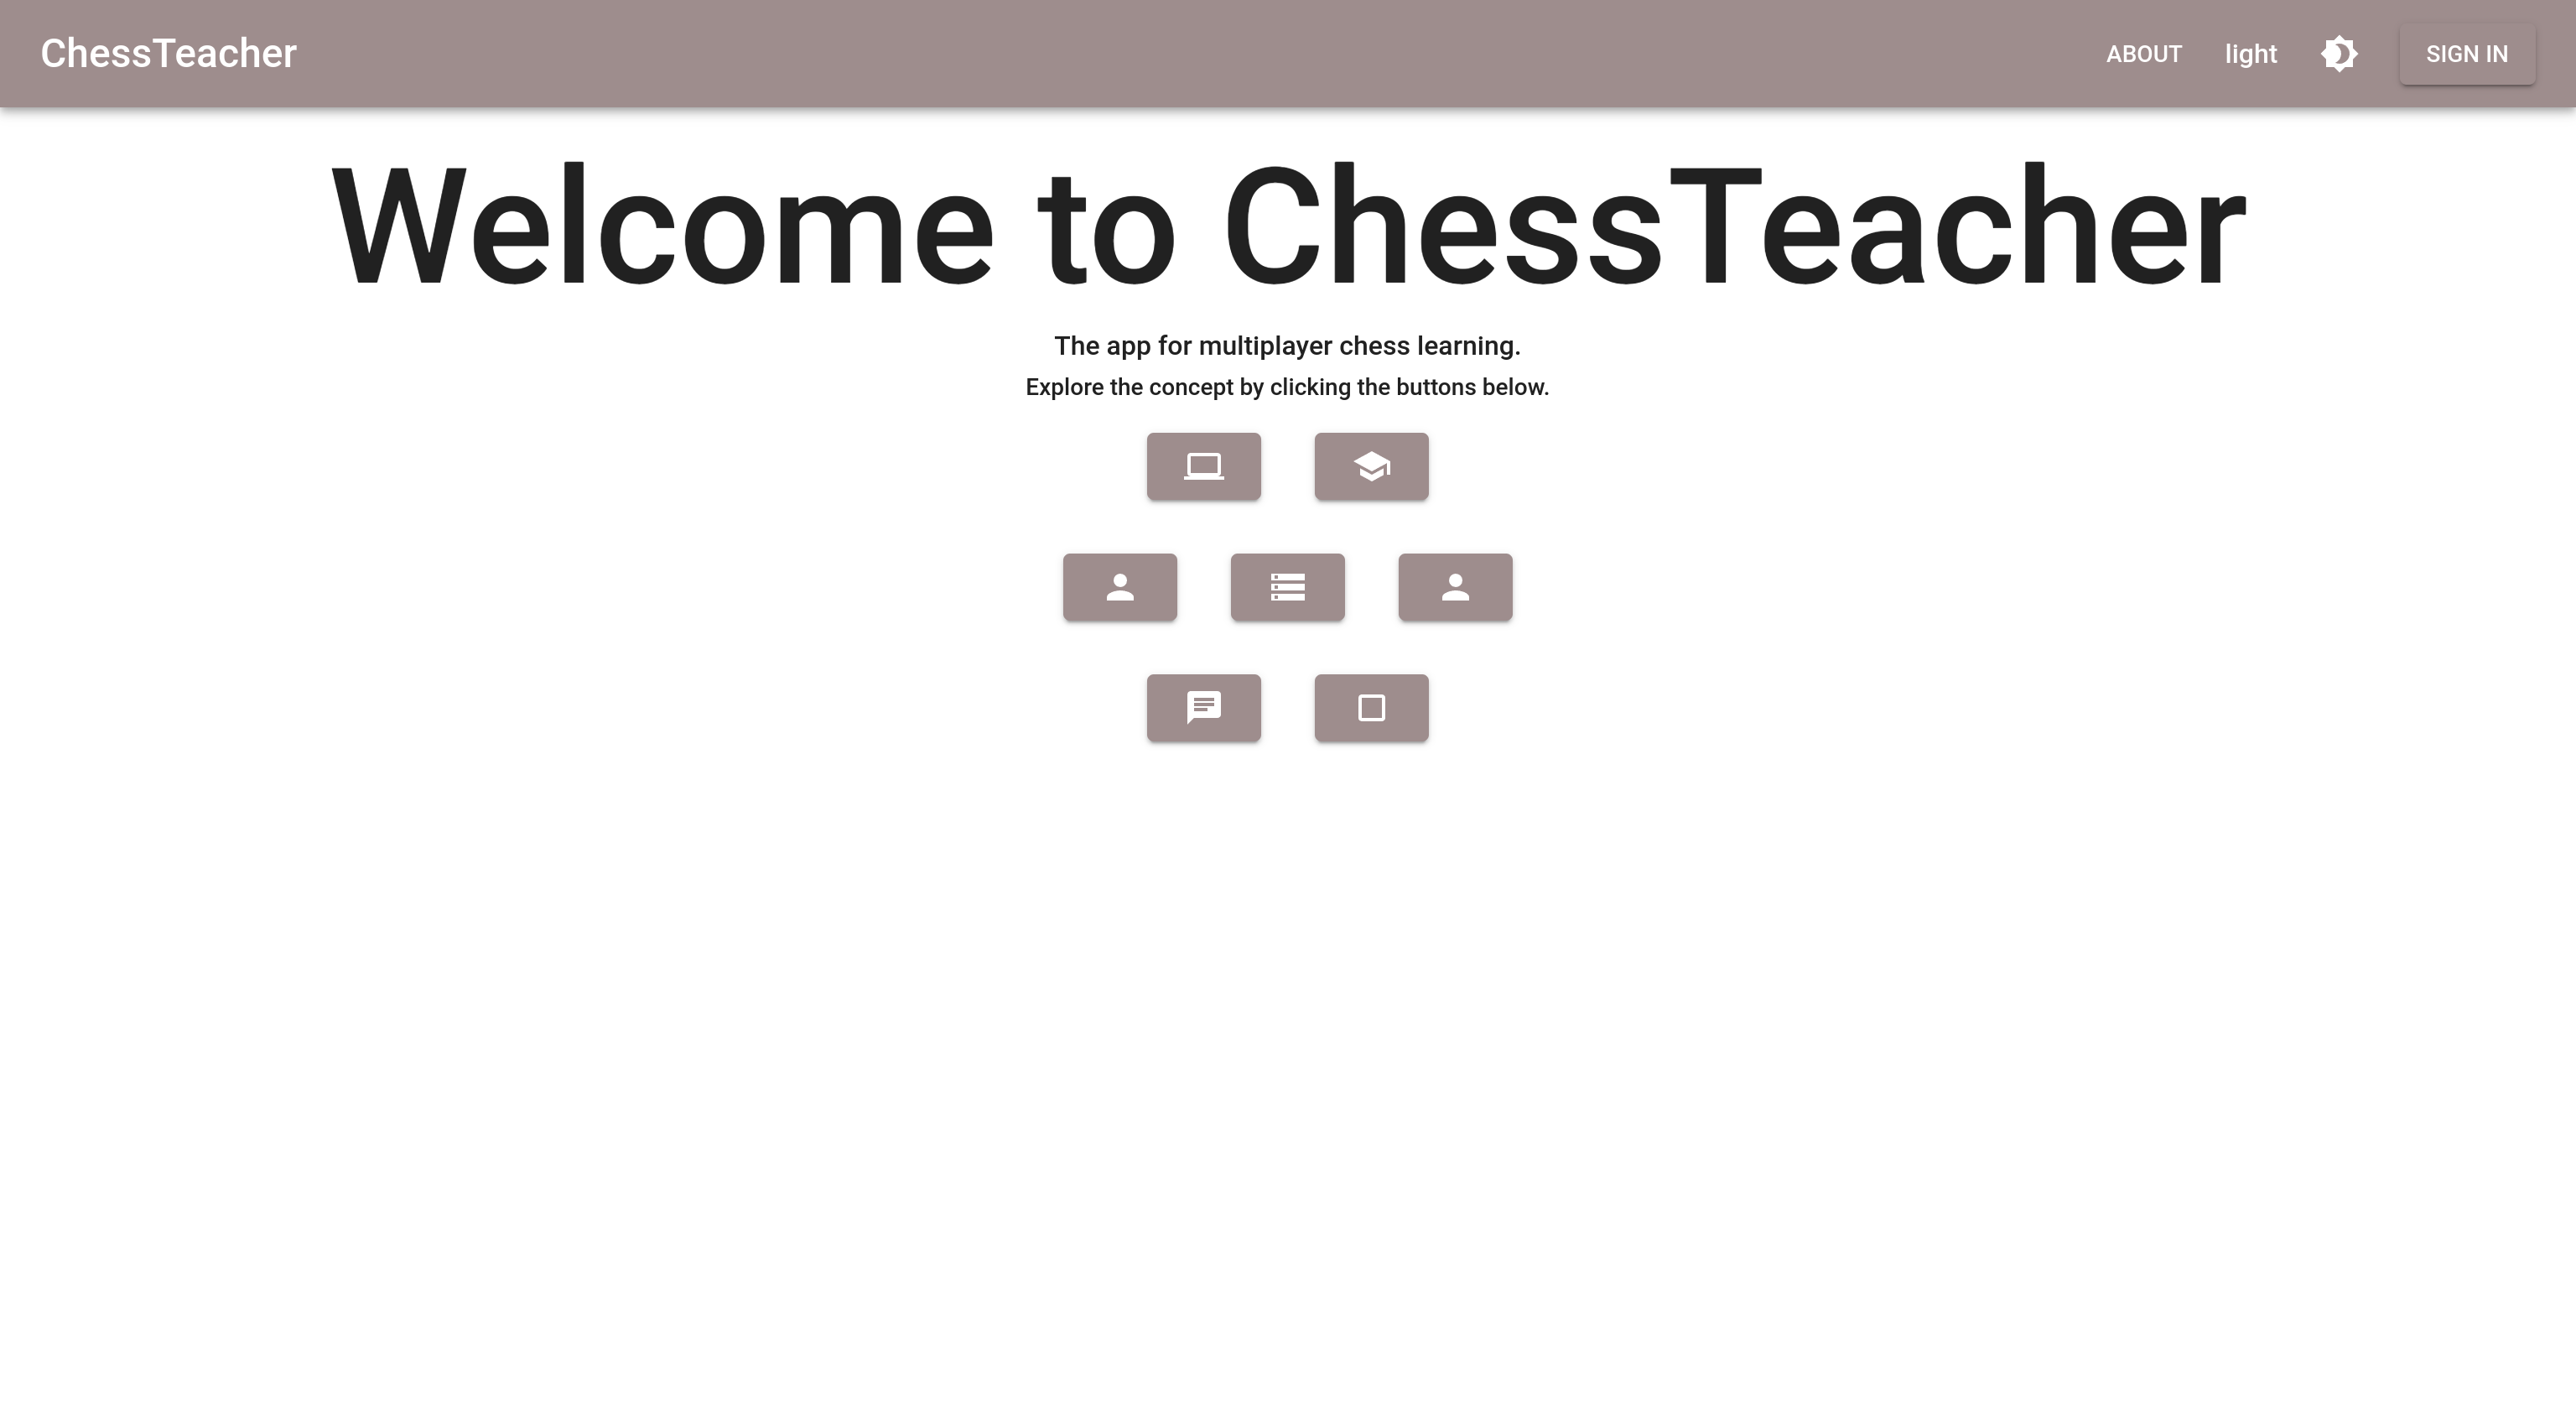
\includegraphics[width=1\textwidth]{frontend-home}}
    \caption{The landing page of the website.}\label{fig:home}
\end{figure}

\begin{figure}[H]
    \centering
    \setlength{\fboxsep}{0pt}
    \fbox{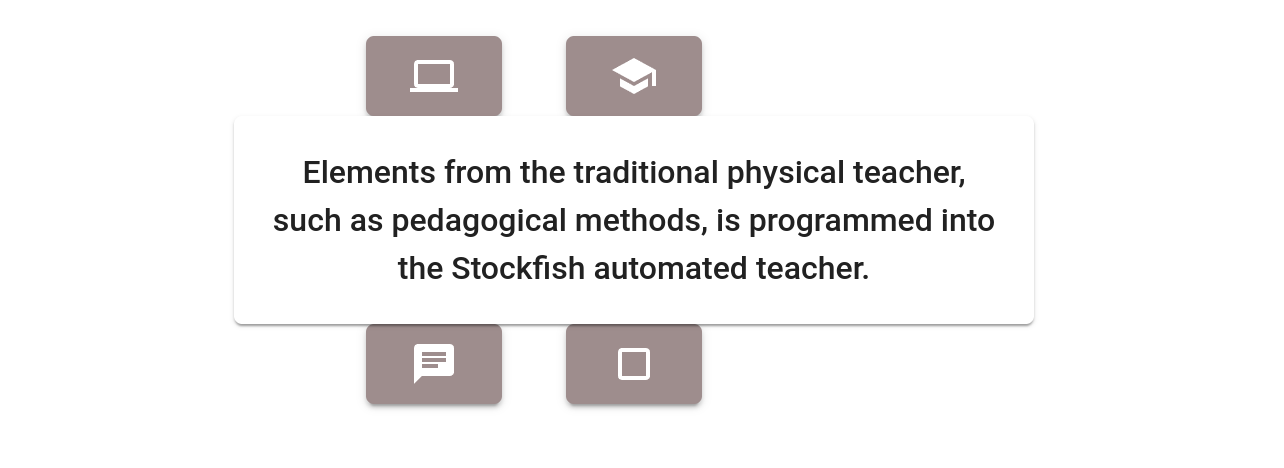
\includegraphics[width=1\textwidth]{frontend-home-info}}
    \caption{More info upon clicking on the buttons.}\label{fig:home-info}
\end{figure}
% textidote: ignore end

To access the game lobby, the user first has to log in.
The login system is based on Firebase Authentication, which was selected for its easy and secure login process.
The user can use their existing Google account to log in, which negates the need for creating a new account.
This makes the login process quick and easy.
To log in, the user has to click on the ``Sign in'' button in the top right corner of the website.
The login screen can be seen in Figure~\ref{fig:login}.

% textidote: ignore begin
\begin{figure}[H]
    \centering
    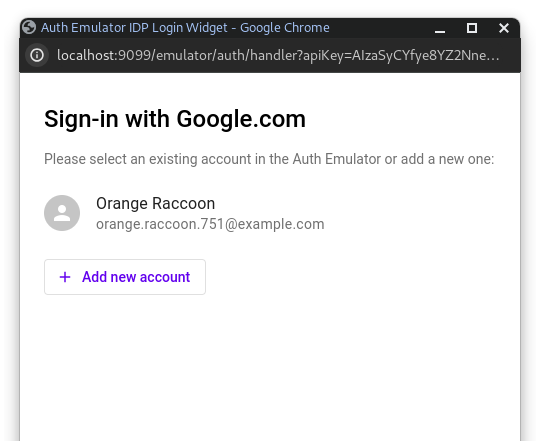
\includegraphics[width=0.8\textwidth]{frontend-login}
    \caption{The Google Authentication prompt when logging in.}\label{fig:login}
\end{figure}
% textidote: ignore end

Once the user is authenticated, the home page will lead to the lobby listing, rather than the landing page.
The lobby listing is a list of all the available games that the user can join.
As more users join the website, the lobby listing will be populated with more games, but during development, the lobby
listing is empty, as seen in Figure~\ref{fig:lobby-empty}.

Anyone can create a new game by clicking on the green ``Create New Match'' button in the top right corner of the
listings.
This will create a new entry to the lobby, as seen in Figure~\ref{fig:lobby-game}.
Once a game is created, a different user can join the game by clicking on the green ``Join'' button in the game's entry.
The creator will get a notification, which can be seen in Figure~\ref{fig:lobby-join}.
It will appear in the bottom right corner of the screen, and it serves to inform the creator that someone has joined
their game and that the game can now start.
The notification was added to improve the user experience, as the creator would otherwise have no other way of knowing
that someone has joined without checking it manually.
Both players will have to open the game by clicking on the ``View'' button, which will replace the ``Join'' button once
the second player has joined.
Other players can spectate the game by clicking that same button.
The team wanted to add a spectating option to the game, because it would allow for a better learning experience, as
spectators can support the players similar to how the chess engine does.

% textidote: ignore begin
\begin{figure}[H]
    \centering
    \setlength{\fboxsep}{0pt}
    \fbox{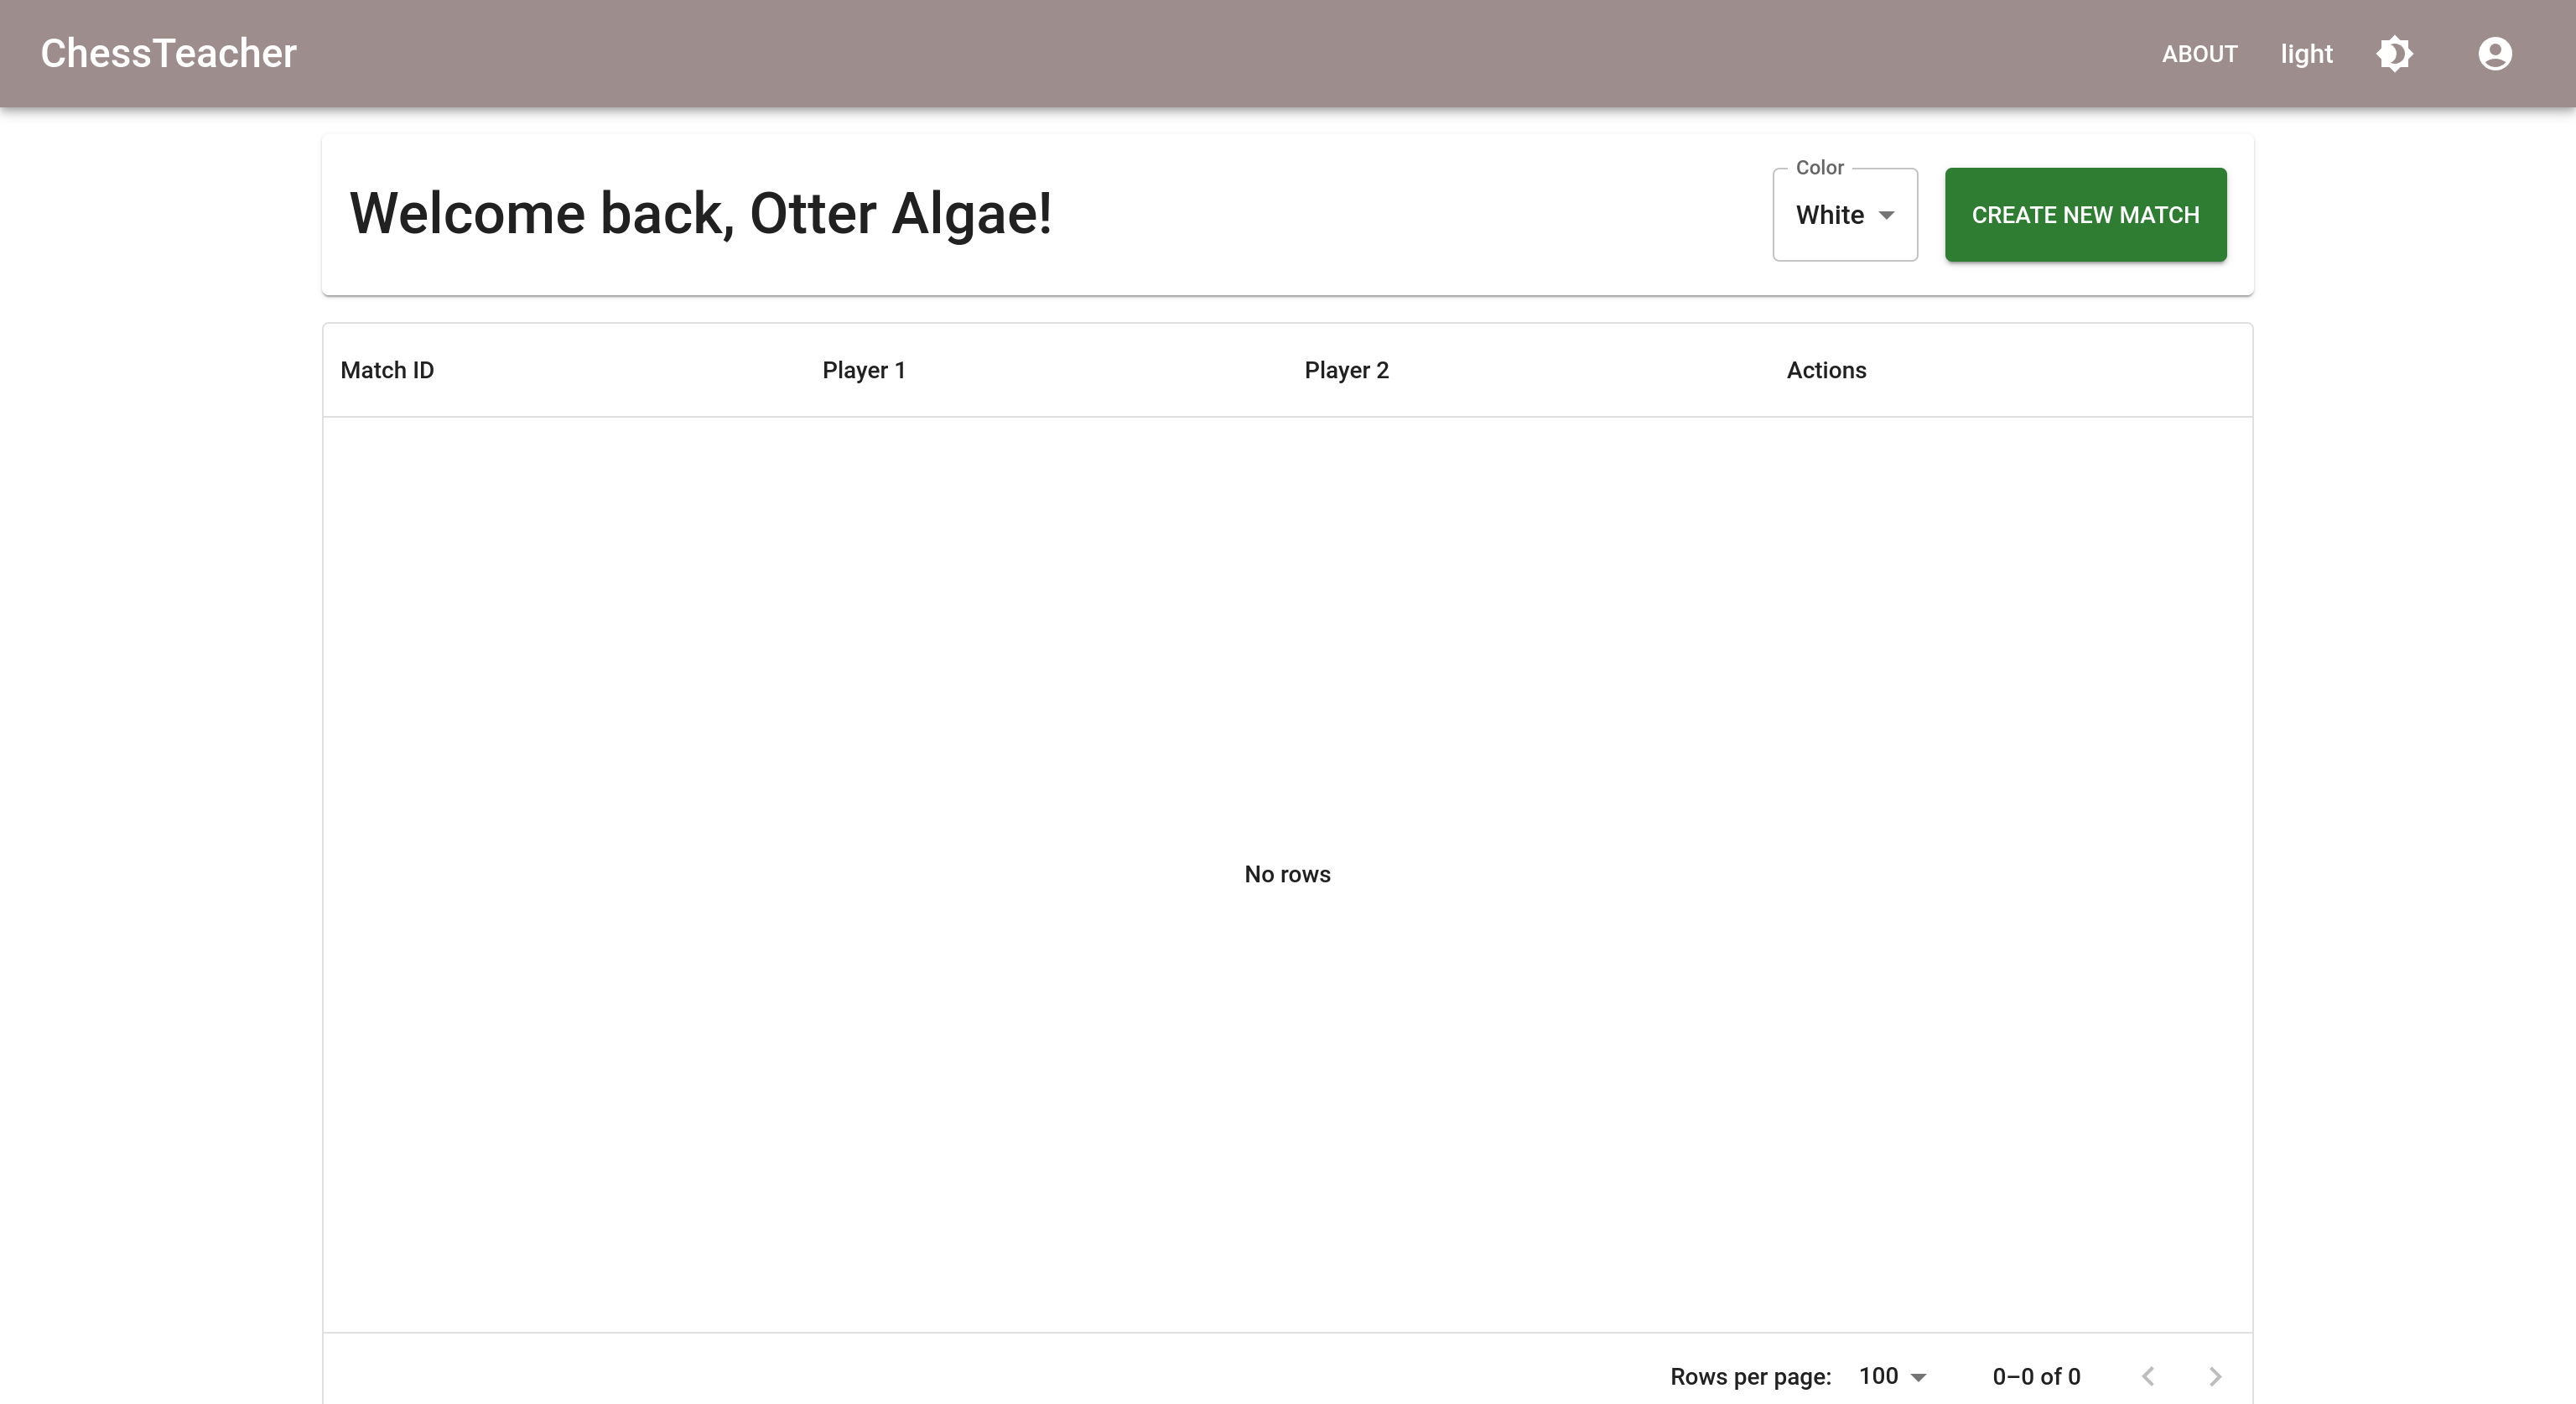
\includegraphics[width=1\textwidth]{frontend-lobby-empty}}
    \caption{The lobby listing of the website.}\label{fig:lobby-empty}
\end{figure}

\begin{figure}[H]
    \centering
    \setlength{\fboxsep}{0pt}
    \fbox{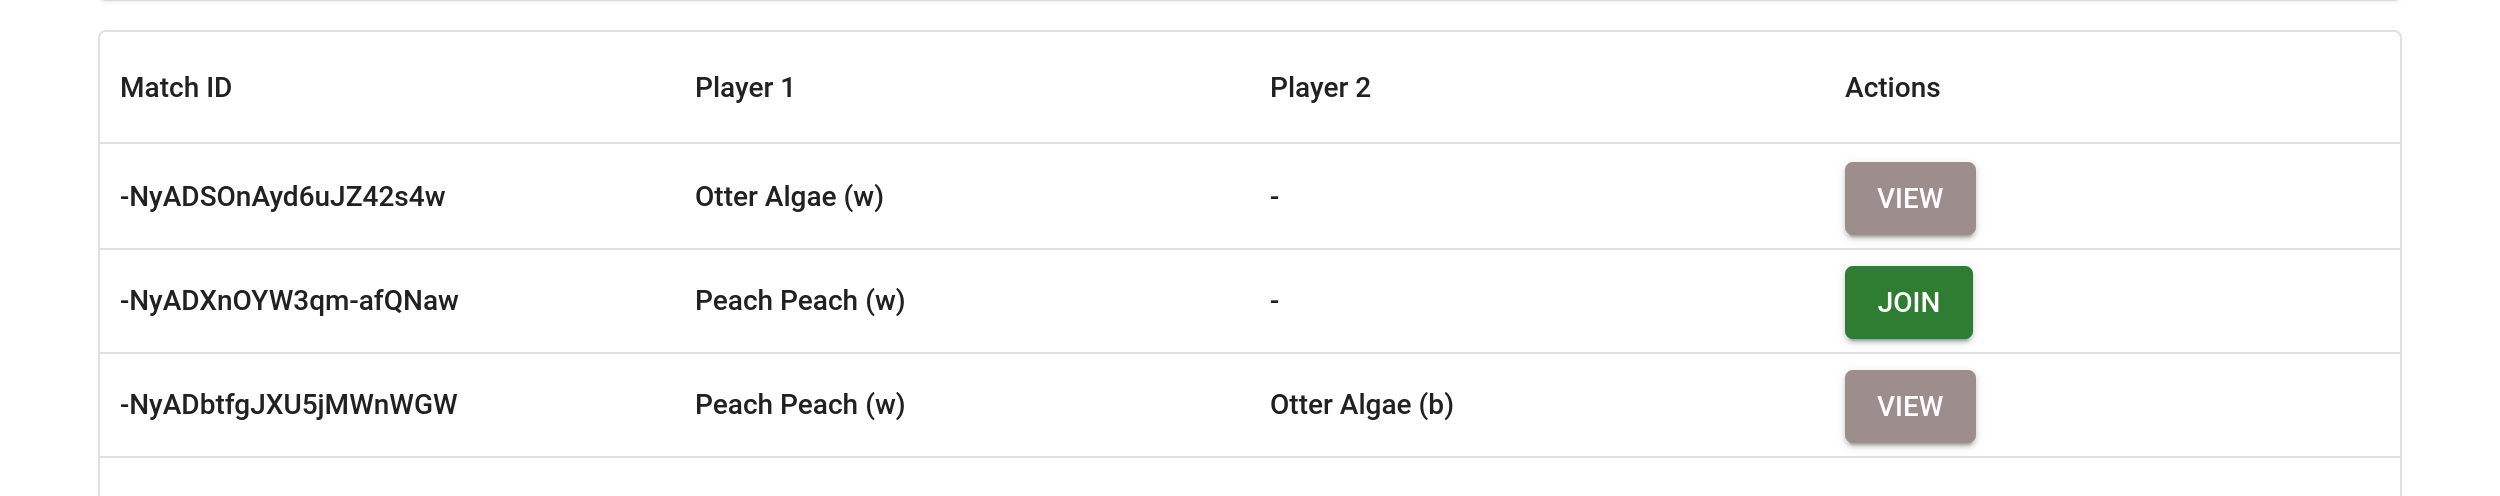
\includegraphics[width=1\textwidth]{frontend-lobby-game}}
    \caption{A game entry in the lobby.}\label{fig:lobby-game}
\end{figure}

\begin{figure}[H]
    \centering
    \setlength{\fboxsep}{0pt}
    \fbox{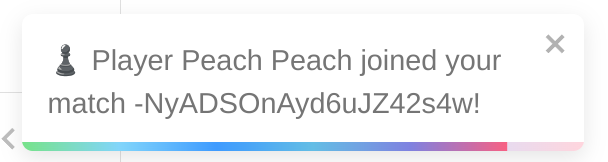
\includegraphics[width=0.7\textwidth]{frontend-lobby-join}}
    \caption{Notification when another player joins the game.}\label{fig:lobby-join}
\end{figure}
% textidote: ignore end

Once in-game, the players are greeted with a chessboard occupying the majority of the screen, and a chat window to the
right of it, as seen in Figure~\ref{fig:game}.
The chessboard is the biggest element on the screen, as it is the main focus of the website, with the chat always
visible to the players.
The two players can take turns making moves, and the engine will provide feedback on the moves, as seen in
Figure~\ref{fig:game-chat}.
The engine gives both players the three best moves they can play on their turn.
Players and spectators can also chat with each other in the chat window.

% textidote: ignore begin
\begin{figure}[H]
    \centering
    \setlength{\fboxsep}{0pt}
    \fbox{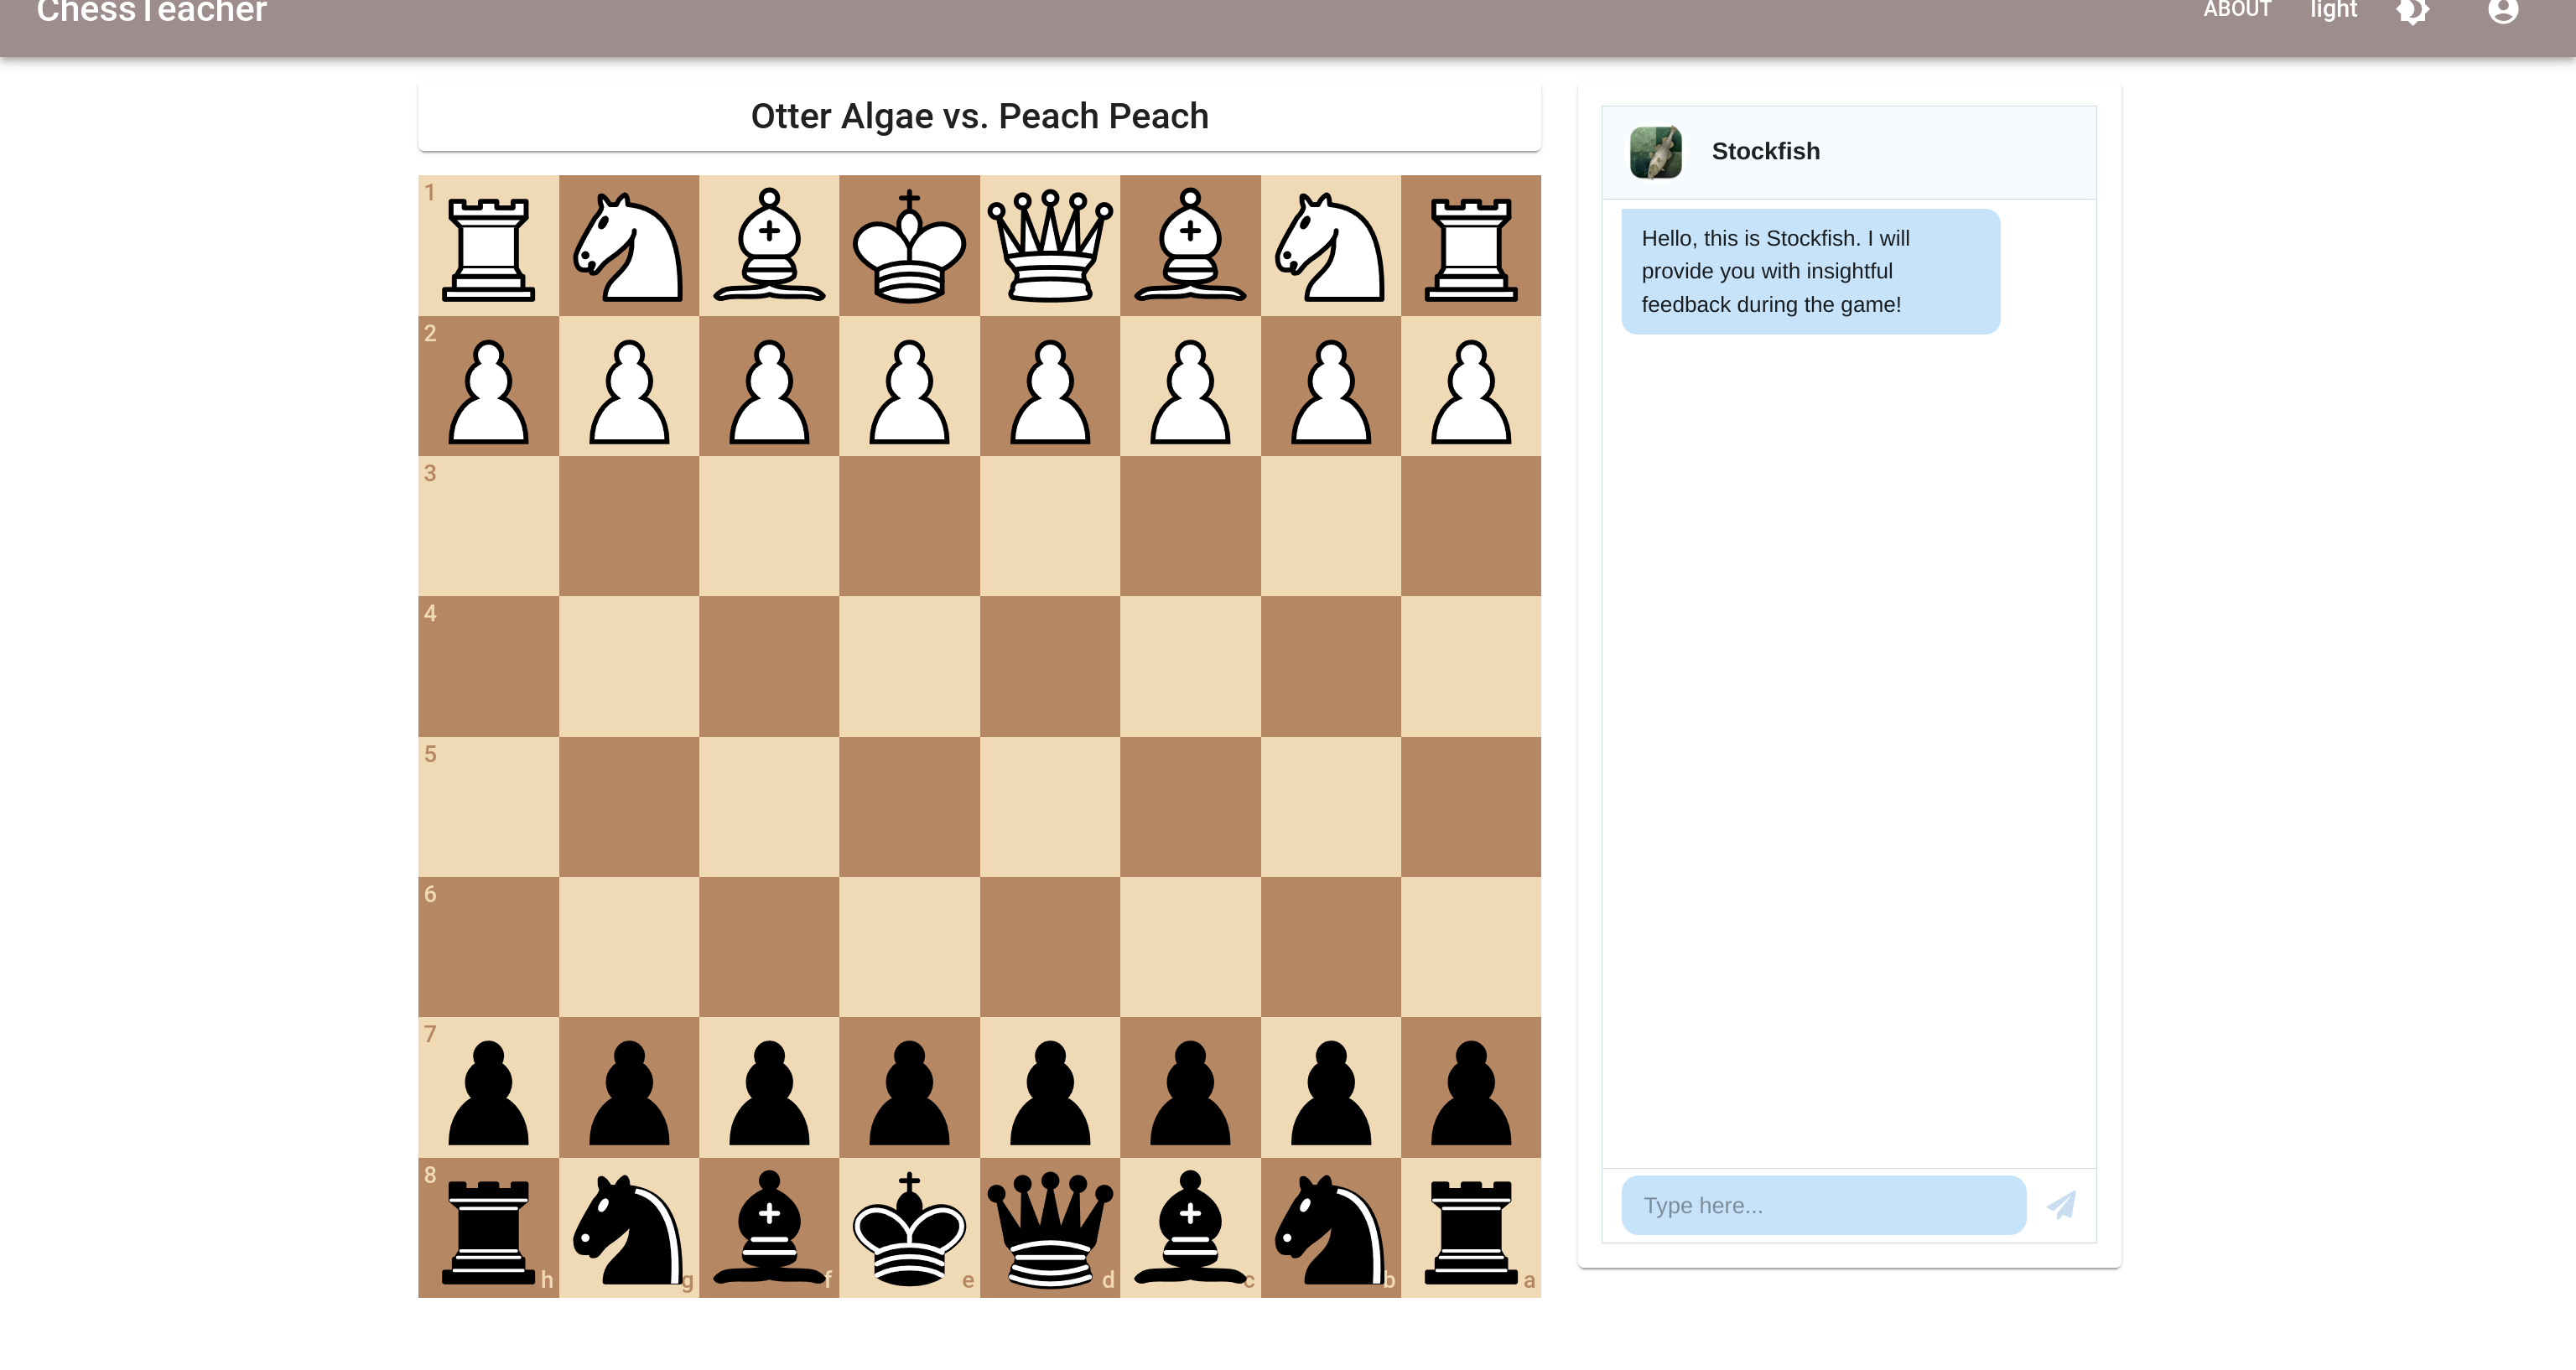
\includegraphics[width=1\textwidth]{frontend-game}}
    \caption{The in-game interface of the website.}\label{fig:game}
\end{figure}

\begin{figure}[H]
    \centering
    \setlength{\fboxsep}{0pt}
    \fbox{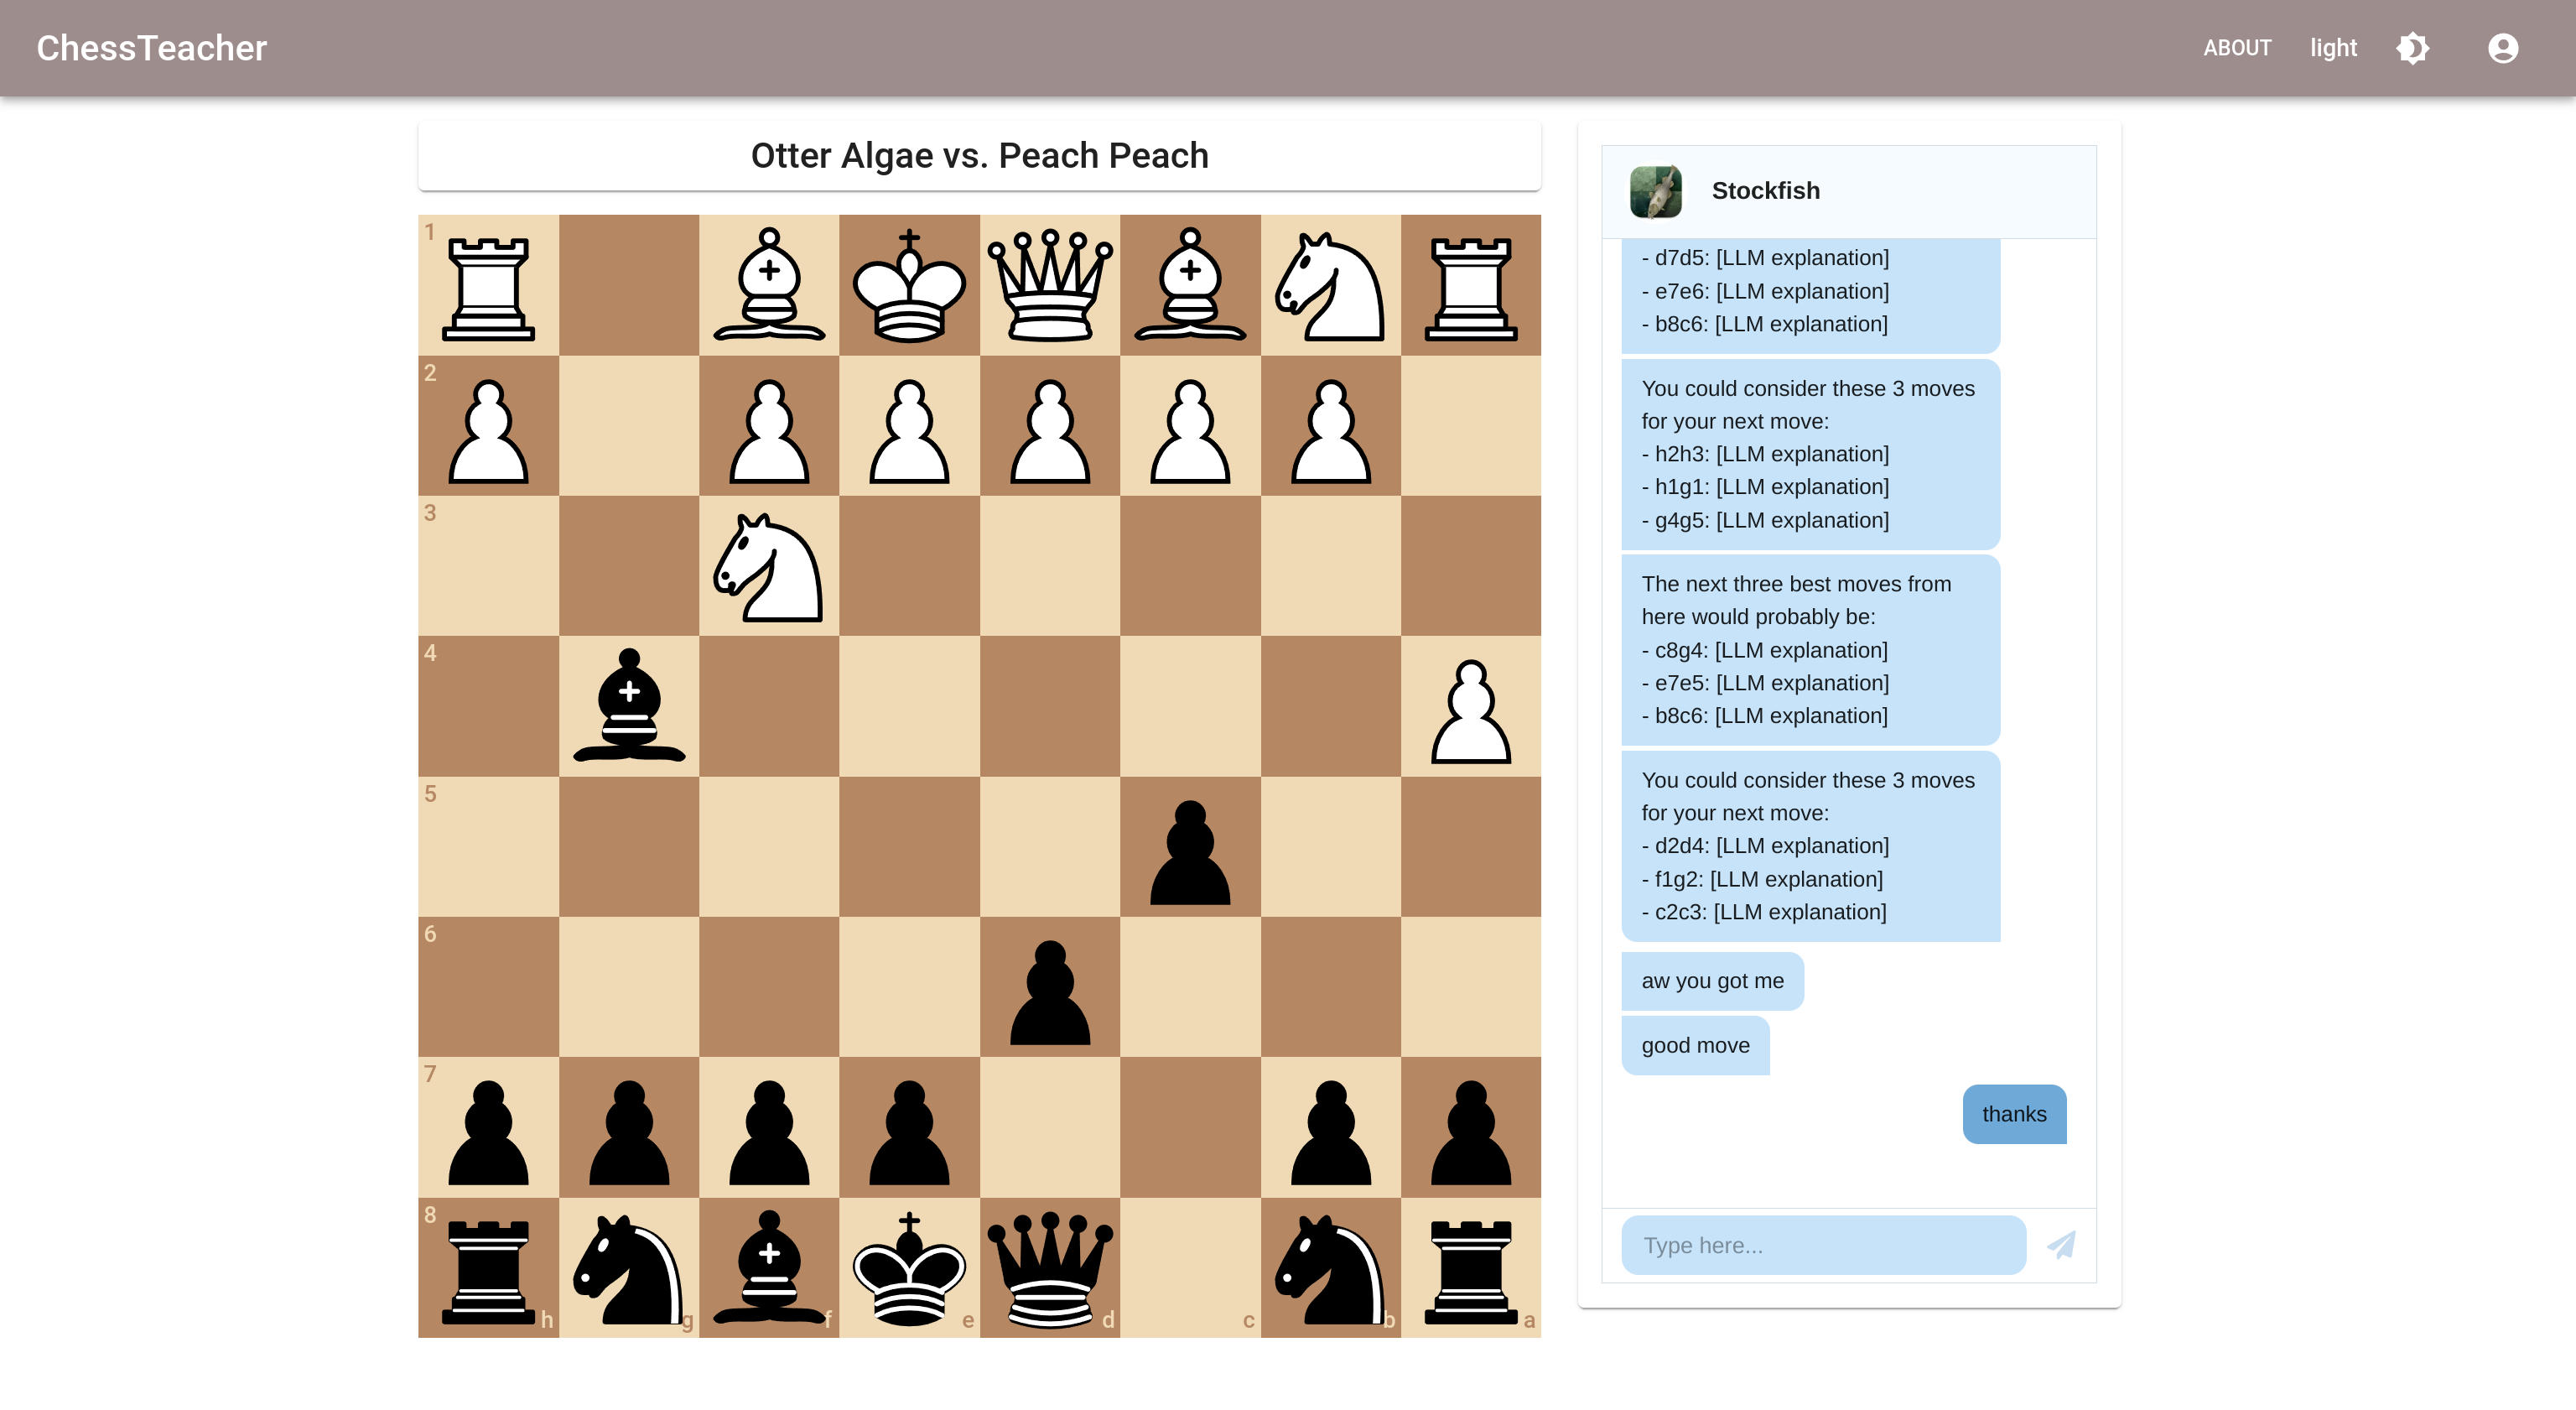
\includegraphics[width=1\textwidth]{frontend-game-chat}}
    \caption{A conversation between the players and stockfish.}\label{fig:game-chat}
\end{figure}
% textidote: ignore end

The website also has a dark mode, which can be toggled by clicking on the sun icon in the top right corner of the
website.
The option to change between light and dark mode was added to improve the user experience, as some users might prefer
one over the other.
The default mode is set to the user's system preference, but the user can change it to their liking.
The dark mode can be seen in Figure~\ref{fig:game-dark}.

% textidote: ignore begin
\begin{figure}[H]
    \centering
    \setlength{\fboxsep}{0pt}
    \fbox{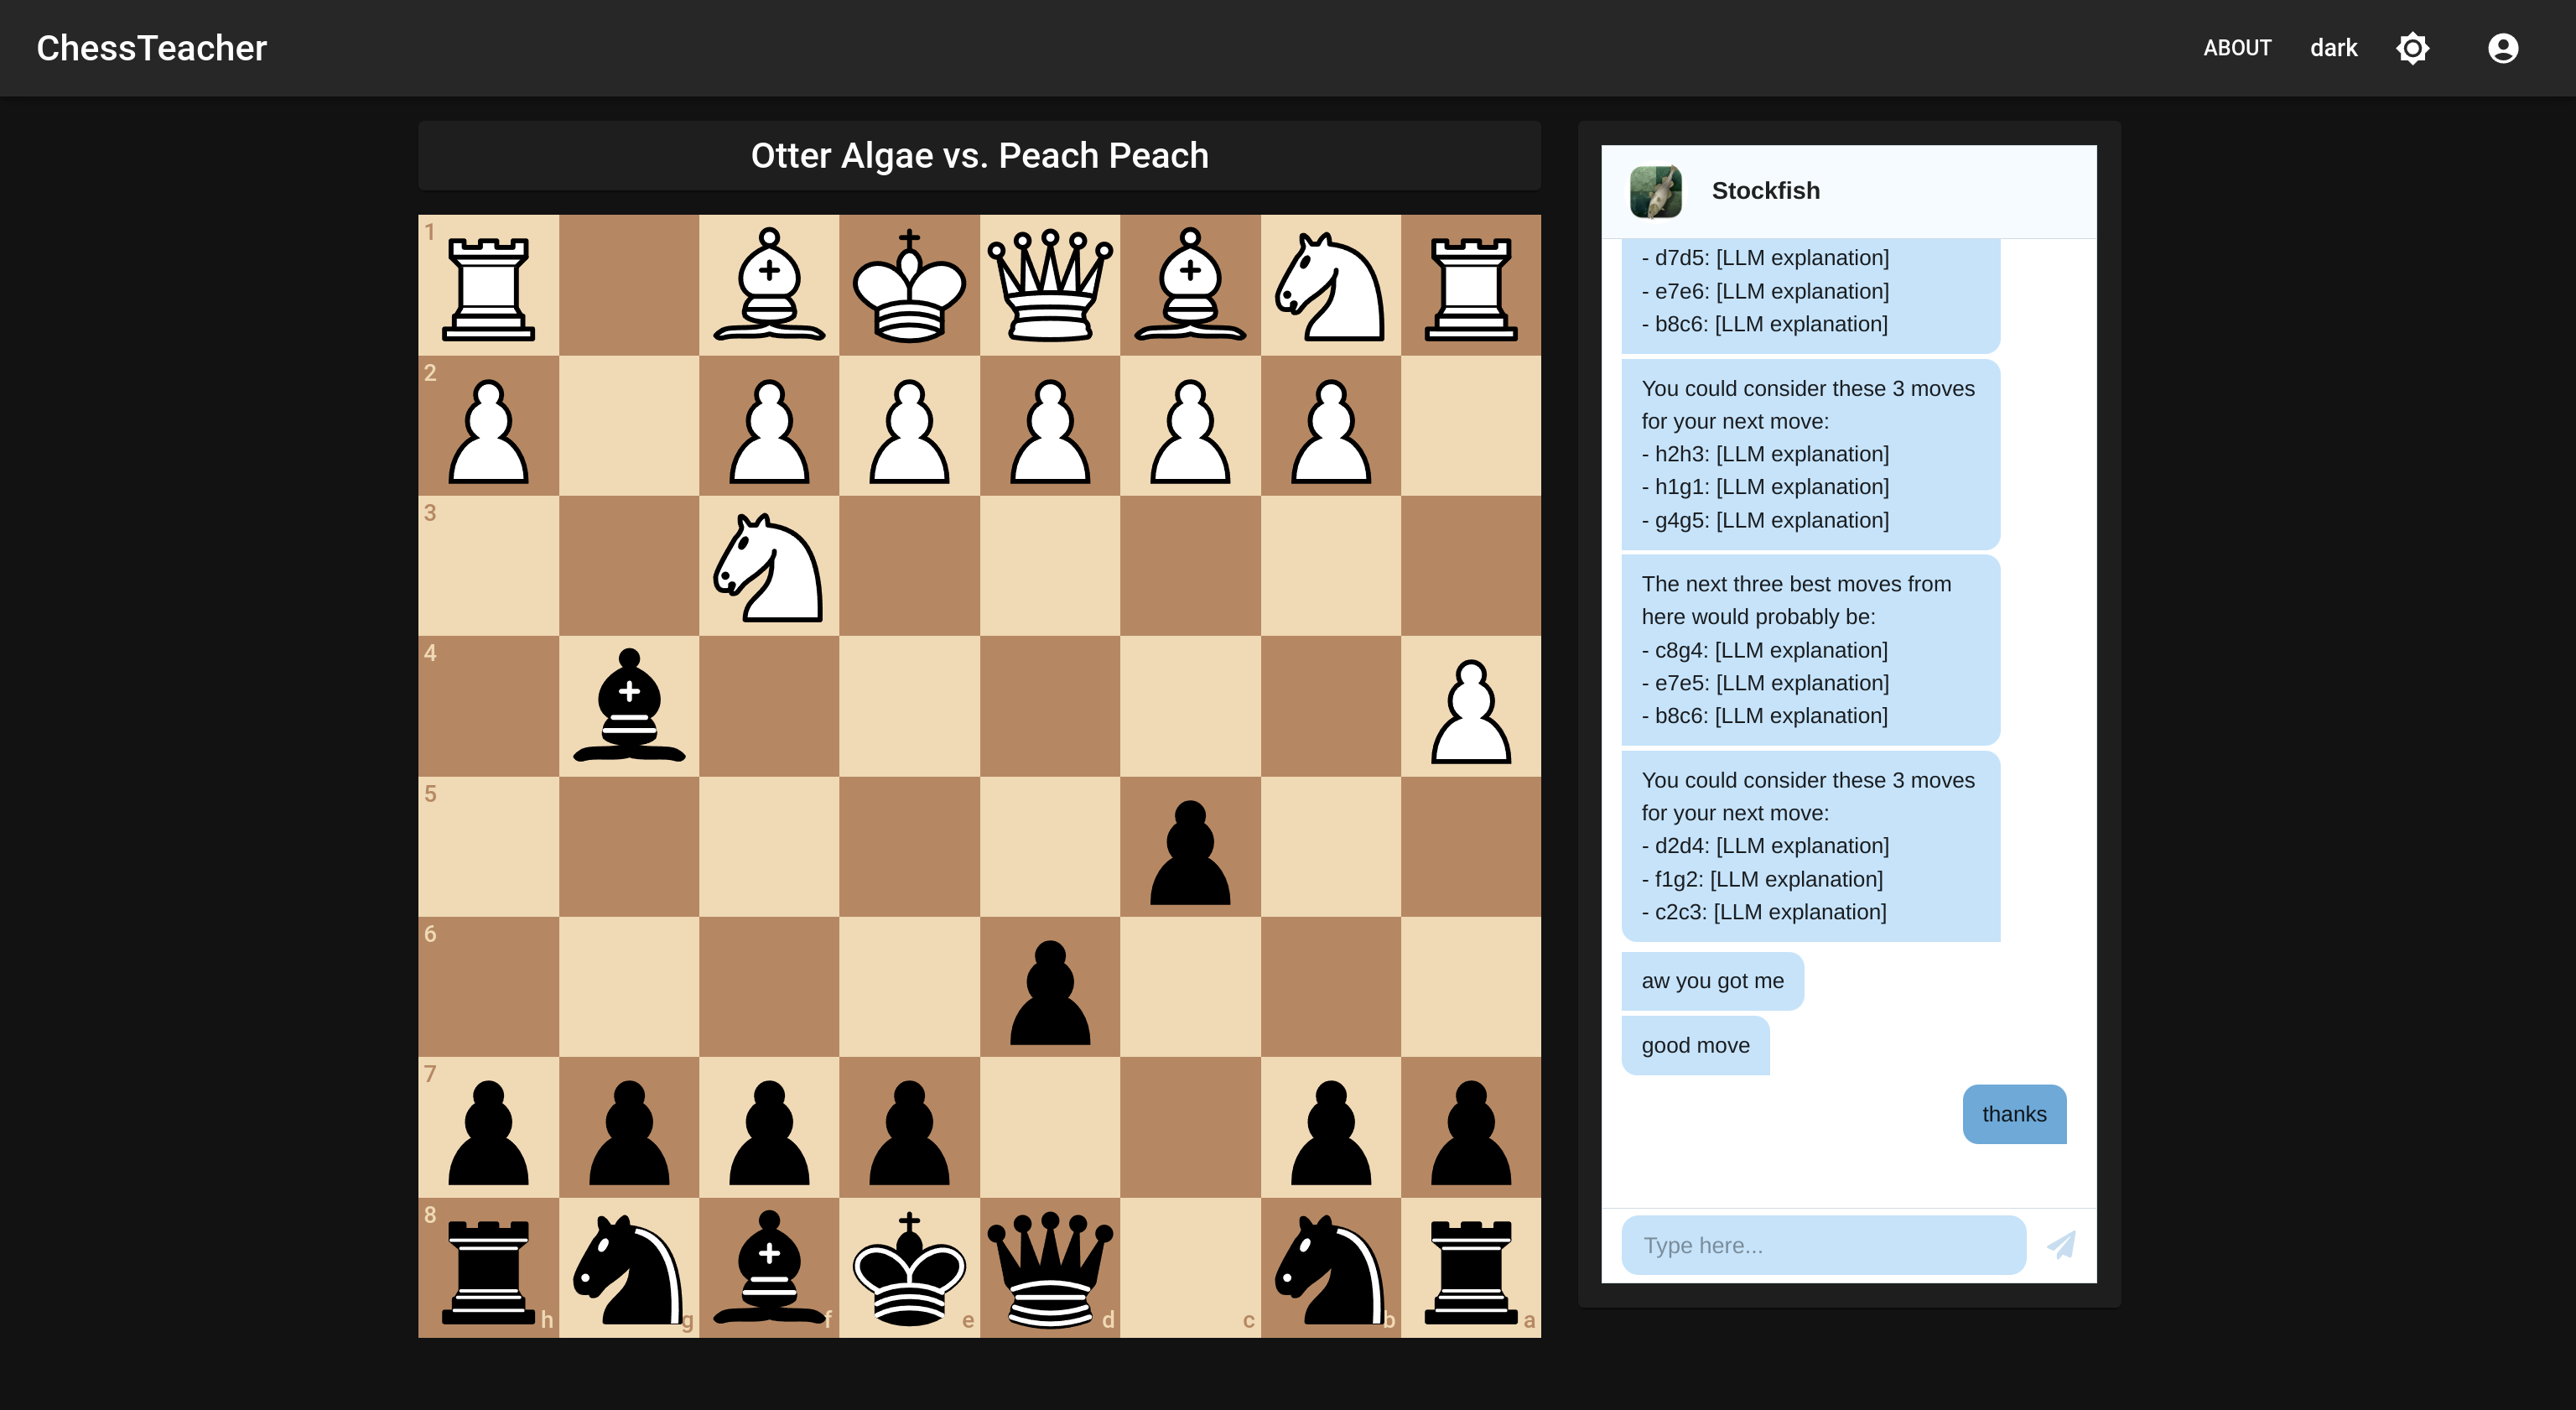
\includegraphics[width=1\textwidth]{frontend-game-dark}}
    \caption{The look of the website in dark mode.}\label{fig:game-dark}
\end{figure}
% textidote: ignore end

Apart from the lobby and the game interface, the website also has an account page, where the user can see their
personal information.
The account page can be seen in Figure~\ref{fig:account}.
It can be accessed by clicking on the user icon on the top right once logged in, and then clicking on ``Account''.
The profile picture is taken from the user's Google account, and if they don't have a picture, their initials will be
displayed instead.

% textidote: ignore begin
\begin{figure}[H]
    \centering
    \setlength{\fboxsep}{0pt}
    \fbox{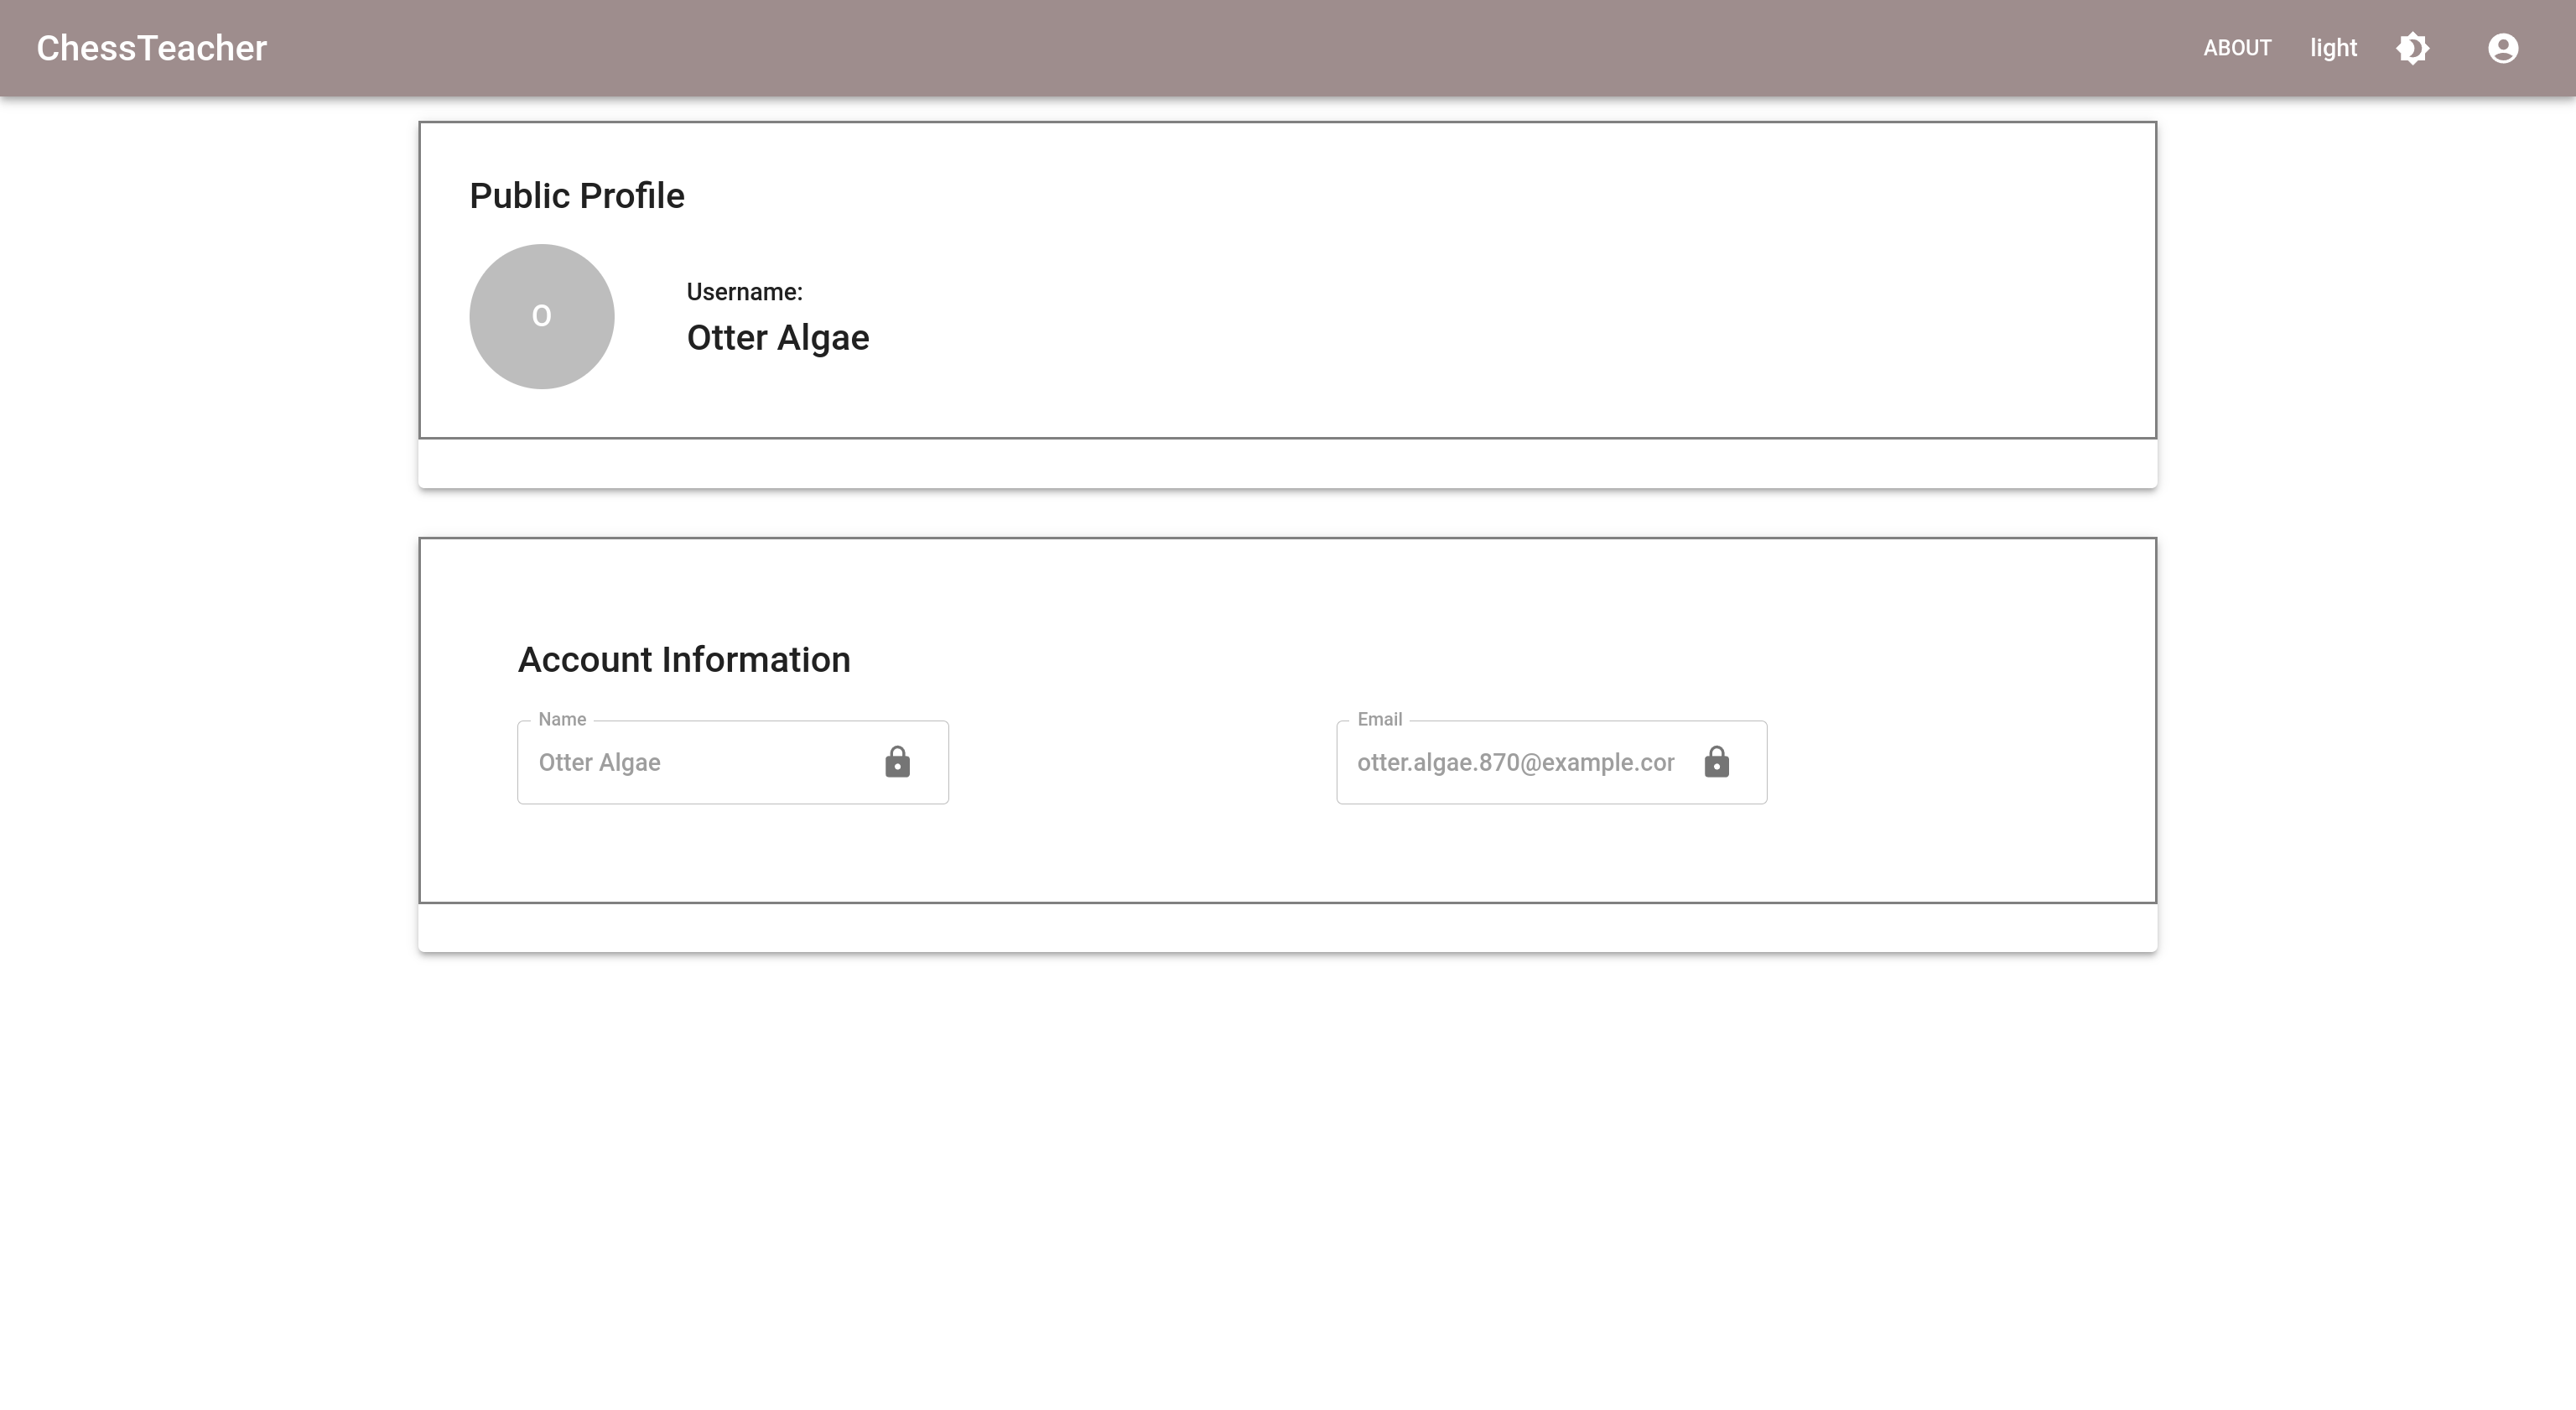
\includegraphics[width=1\textwidth]{frontend-account}}
    \caption{The account page of the website.}\label{fig:account}
\end{figure}
% textidote: ignore end

There is also an about page, which can be accessed by clicking on the ``About'' button on the top right of the
website.
It serves to inform the user about the project and the people behind it.
The page can be seen in Figure~\ref{fig:about}.

% textidote: ignore begin
\begin{figure}[H]
    \centering
    \setlength{\fboxsep}{0pt}
    \fbox{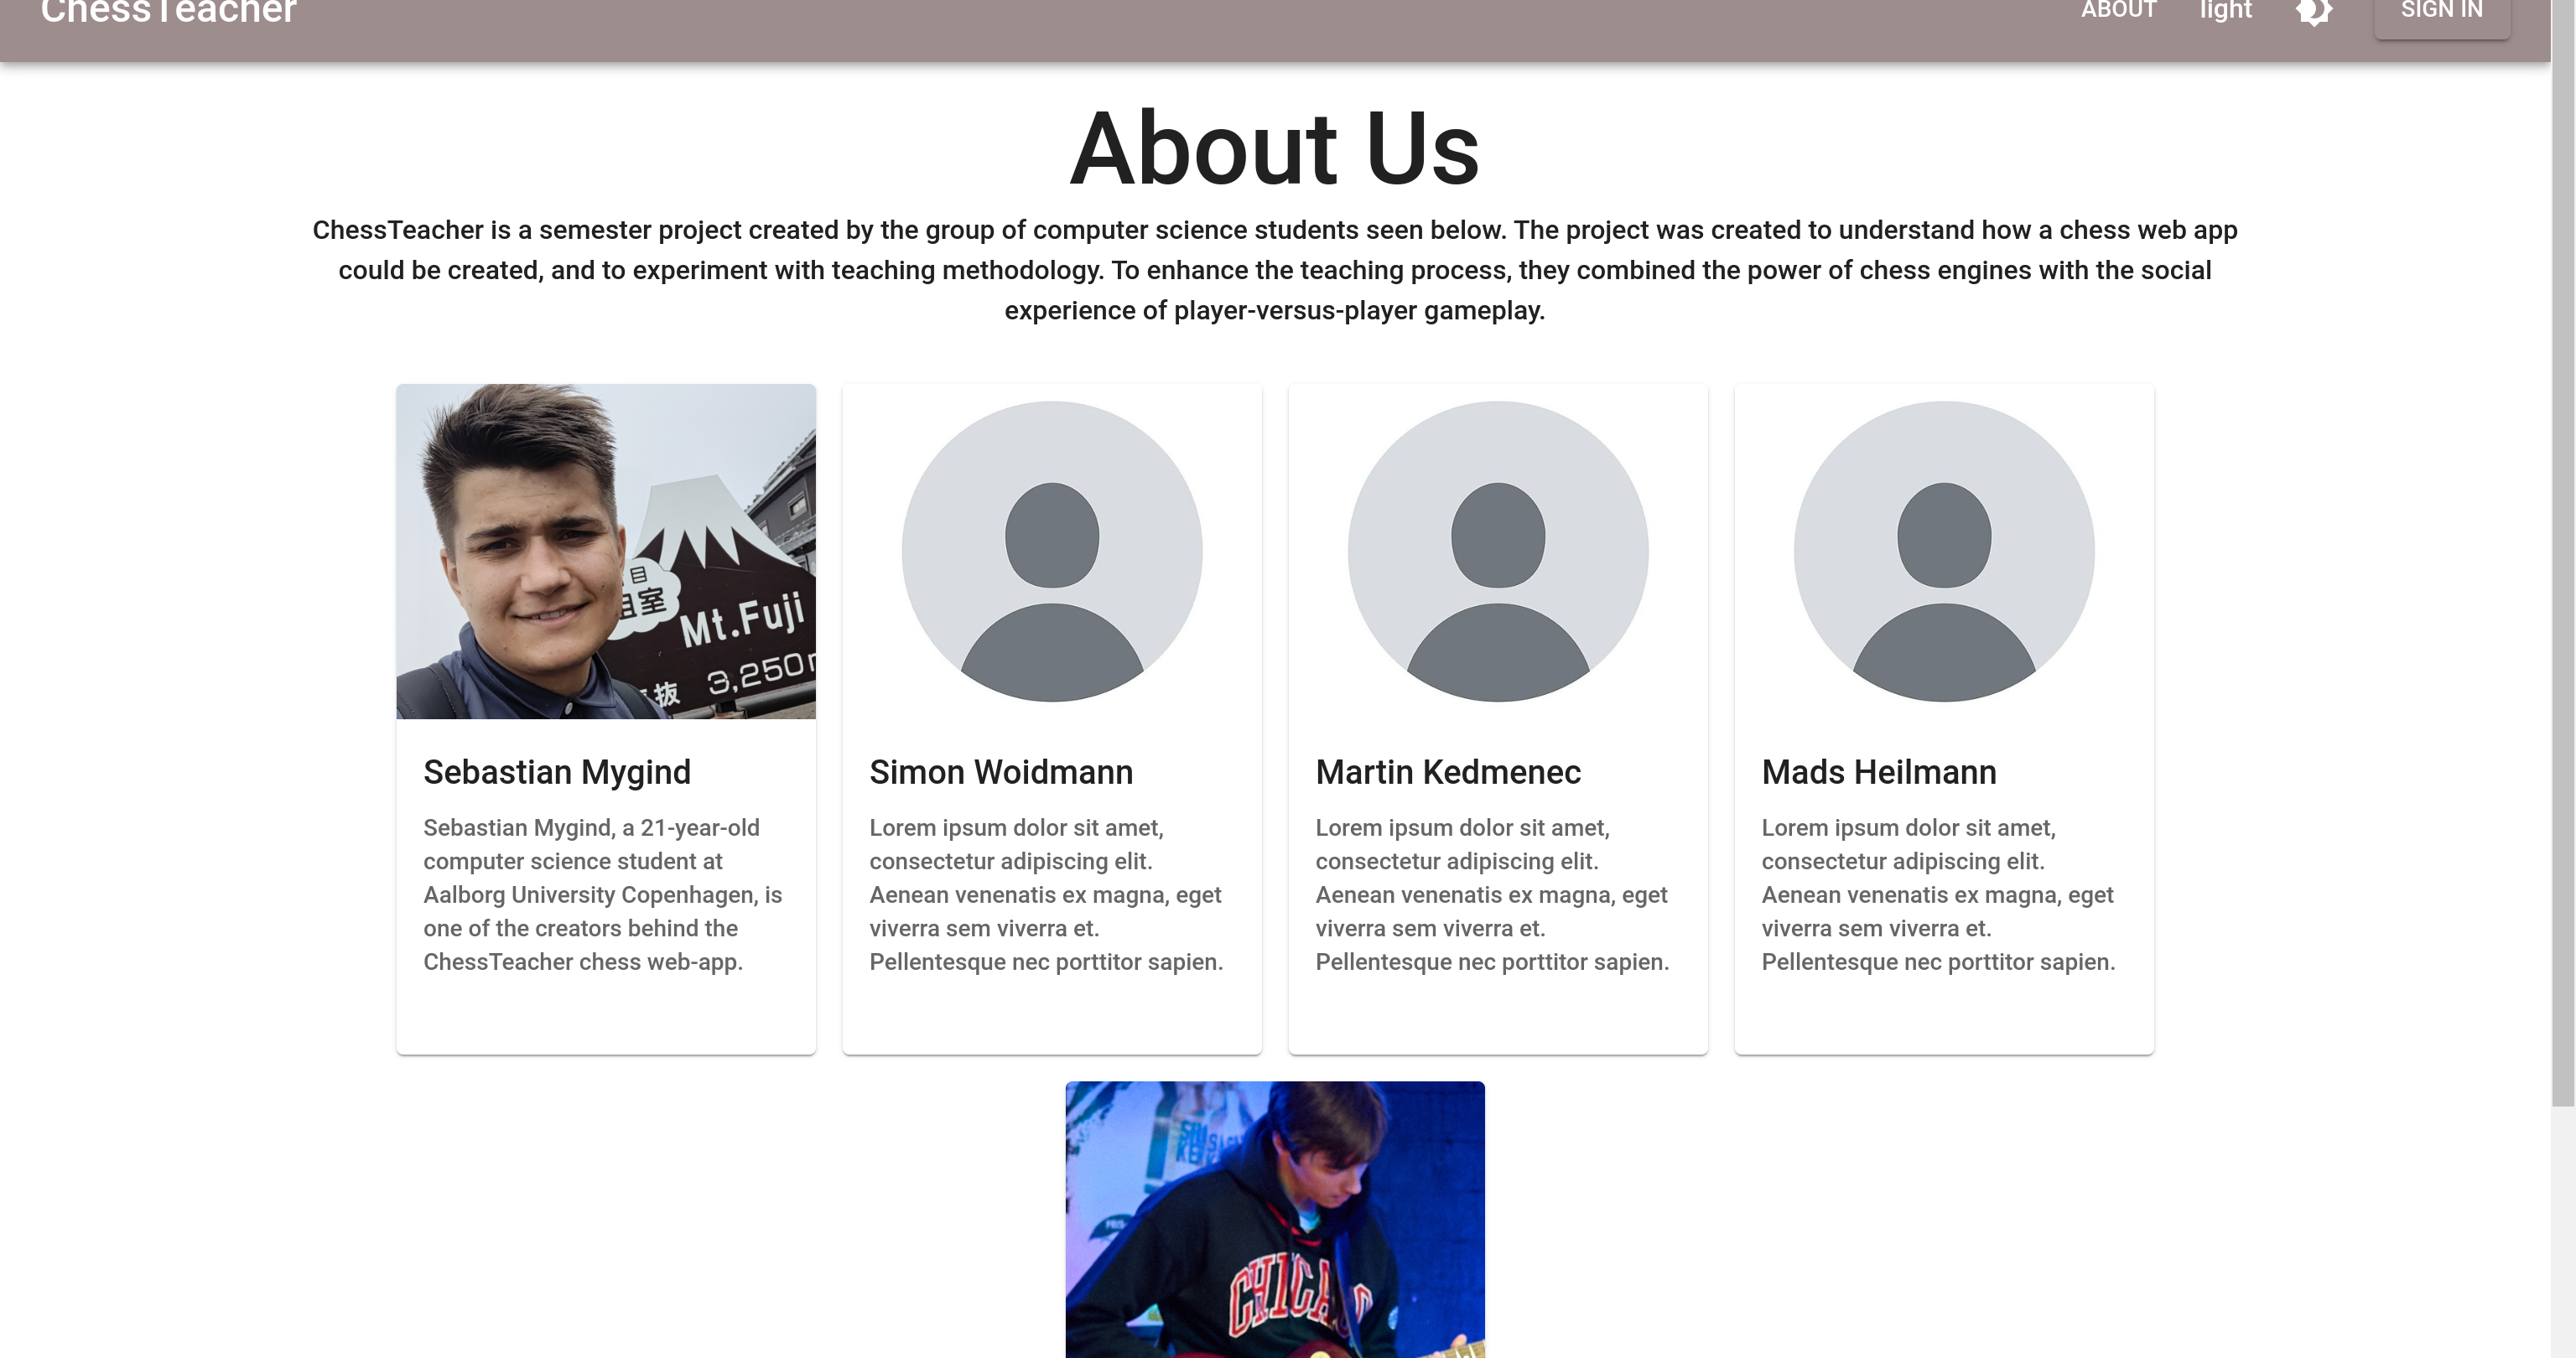
\includegraphics[width=1\textwidth]{frontend-about}}
    \caption{The about page of the website.}\label{fig:about}
\end{figure}
% textidote: ignore end
